\chapter{Color-based Image Segmentation}
\label{chap:segmentation}
\setlength{\fboxsep}{0pt}
\setlength{\fboxrule}{0.2pt}

\lhead{Chapter 5. \emph{Color-based Image Segmentation}}
 

\section{Introduction}

Segmentation is one of the first steps in sky/cloud image analysis. It remains a challenging task because of the non-rigid, feature-less, and poorly-defined structure of clouds, whose shape also changes continuously over time. Thus, classical image segmentation approaches based on shape priors~\cite{wrapper_Jain} are not suitable. Furthermore, the wide range of lighting conditions (direct sunlight to completely covered skies) adds to the difficulty. Therefore, in most cases, color is used as the most discriminatory cue. In the previous Chapter~\ref{chap:colorchannels}, we have provided a systematic analysis of the various color spaces and components. 
In one of our earlier works~\cite{ICIP2015a}, we learnt the semantics of sky/cloud images for an automatic annotation of pixels with three class labels---sky, thin clouds and thick clouds. However, the segmentation results were not promising for thin clouds. Therefore, based on the findings of the previous chapter, we propose a probabilistic color-based image segmentation algorithm in this chapter.



\section{Outline of Our Contribution}
The motivation of this chapter is to propose a robust framework for color-based cloud segmentation under any illumination conditions, including a systematic analysis of color channels. The framework is based on partial least squares (PLS) regression and provides a straightforward, parameter-free supervised segmentation method. We show that our approach is robust and offers a superior performance across two different databases as compared to current state-of-the-art algorithms. Furthermore, it allows annotating each pixel with a degree of \emph{belongingness} to the sky or cloud category, instead of the usual binary labeling.

The main novel contributions of this chapter compared to earlier works include: 

\begin{itemize}
\item Introduction of a large public sky/cloud image database with segmentation masks;
\item Extensive evaluation of color components and selection of appropriate color channels on two different sky/cloud image databases;
\item Robust learning-based framework for sky/cloud segmentation that outperforms existing methods.
\end{itemize}

The rest of this chapter is organized as follows. Section~\ref{sec:prob-segment} discusses our proposed supervised probabilistic segmentation framework. The sky/cloud databases used for evaluation, including our newly introduced database, are presented in Section~\ref{sec:database}. Section~\ref{sec:result-segment} presents the experimental evaluation of the segmentation framework. We extend our discussion to High Dynamic Range (HDR) images in Section~\ref{sec:HDRI-segment}. Section~\ref{sec:conc} concludes this chapter.


\section{Probabilistic Segmentation}
\label{sec:prob-segment}
Using statistical tools, we identify the most discriminative color channels for cloud segmentation. Out of $16$ color channels, the best performing color channels may be subsequently used as discriminatory feature $\mathbf{X}^{f}_{i}$ in the segmentation framework. 

Our objective is to predict the label of a pixel as either sky or cloud, given a set of training images with manually annotated ground truths. We formulate this task of sky/cloud image segmentation in a probabilistic manner using PLS regression. Both Principal Component Analysis (PCA) and PLS are based on the same underlying motivation, namely to extract components that accounts for maximum variation in input data. Unlike alpha matting, we do not assume that a particular pixel is a linear combination of two classes -- \emph{sky} and \emph{cloud}.

We start with the assumption that the sky/cloud segmentation problem is dependent on a large number of explanatory independent variables (color channels in this case). Using dimensionality reduction techniques like PCA, we observe the degree of correlation amongst the variables and the amount of variance captured. PCA provides this information based only on the independent input color channels and project the data into new sets of orthogonal axes. In PLS however, both the input color channels and the output labels (sky/cloud) are considered. Using a set of manually defined ground truth images, we model the relationship between the input features and the output label. In the testing stage, we use this estimated model to predict the output labels of the pixels of a given test image.

Suppose, for a sample $\mathbf{X}_{i} \in {\rm I\!R}^{m \times n}$, the feature vector is denoted by $\mathbf{X}^{f}_{i} \in {\rm I\!R}^{mn \times k}$ and the corresponding binary ground-truth image as $\mathbf{Y}_{i} \in {\rm I\!R}^{mn \times 1}$.  The feature vector $\mathbf{X}^{f}_{i}$ consists of $k$ color channels from the set of $16$ color channels. We decompose the feature vector $\mathbf{X}^{f}_{i}$ and labels $\mathbf{Y}_{i}$ as 
\begin{align}
\mathbf{X}^{f}_{i} = \mathbf{T}_{i}\mathbf{P}_{i}^{T} + \mathbf{E}_{i},\\
\mathbf{Y}_{i} = \mathbf{U}_{i}\mathbf{Q}_{i}^{T} + \mathbf{F}_{i},
\label{eq:pls1}
\end{align}
where $\mathbf{T}_{i} \in {\rm I\!R}^{mn \times p}$ and $\mathbf{U}_{i} \in {\rm I\!R}^{mn \times p}$ are $p$ extracted latent matrices.  $\mathbf{P}_{i} \in {\rm I\!R}^{k \times p}$ and $\mathbf{Q}_{i} \in {\rm I\!R}^{1 \times p}$ are the loading matrices, and $\mathbf{E}_{i} \in {\rm I\!R}^{mn \times k}$ and $\mathbf{F}_{i} \in {\rm I\!R}^{mn \times 1}$ are the residual matrices. Henceforth, for the sake of brevity and without loss of generality we drop the suffix $i$ in the notations. 

In the generalized partial least squares regression sense, we decompose $\mathbf{X}^{f}$ and $\mathbf{Y}$ so as to maximize the covariance between $\mathbf{T}$ and $\mathbf{U}$~\cite{SIMPLS}.
Under the assumption that the input matrix $\mathbf{X}^{f}$ can be expressed as a linear combination of a few latent variables, we can assume the existence of a linear relationship between $\mathbf{T}$ and $\mathbf{U}$ such that \begin{align}
\label{eq:pls2}
\mathbf{U} = \mathbf{T}\mathbf{D}+\mathbf{H},
\end{align}
where $\mathbf{D} \in {\rm I\!R}^{p \times p}$ is a diagonal matrix and $\mathbf{H}$ is the residual matrix. Combining Eqs.\ (\ref{eq:pls1}) and (\ref{eq:pls2}), we get
\begin{gather}
\label{eq:pls3}
\mathbf{Y}=\mathbf{T}\mathbf{D}{\mathbf{Q}}^{T} + (\mathbf{H}\mathbf{Q}^{T} + \mathbf{F}),\\
\mathbf{Y}=\mathbf{T}\mathbf{C}^{T} + \mathbf{F}^{*},
\end{gather}
where $\mathbf{C}^{T}$ is the matrix of regression coefficients and $\mathbf{F}^{*}$ is the residual matrix. We extract score vectors $\mathbf{t}$ and $\mathbf{u}$ from predictors and response variables respectively, and express as: 
\begin{gather}
\mathbf{t}=\mathbf{Xw},\\
\mathbf{u}=\mathbf{Yc},
\end{gather}
where $\mathbf{w}$ and $\mathbf{c}$ are the corresponding weight vectors of $\mathbf{X}$ and $\mathbf{Y}$. These score vectors are necessary to define the response and predictor variables in the PLS setting. $\mathbf{W}$ represents a set of orthogonal basis vectors, such that $\mathbf{W}=(\mathbf{w}_1, \mathbf{w}_2, \ldots, \mathbf{w}_p)$. From~\cite{Manne1987}, we can express the regression coefficient matrix as 
\begin{align}
\label{eq:pls4}
\mathbf{T} = \mathbf{X}\mathbf{W}(\mathbf{P}^{T}\mathbf{W})^{-1}.
\end{align}

Using Eqs.~(\ref{eq:pls3}) and (\ref{eq:pls4}), we get
\begin{gather}
\label{eq:pls5}
\mathbf{Y}=\mathbf{X}\mathbf{W}(\mathbf{P}^{T}\mathbf{W})^{-1}\mathbf{C}^{T} + \mathbf{F}^{*}, \\
\label{eq:pls6}
\mathbf{Y}=\mathbf{XB} + \mathbf{F}^{*},
\end{gather}
where $\mathbf{B}=\mathbf{W}(\mathbf{P}^{T}\mathbf{W})^{-1}\mathbf{C}^{T}$ represents the matrix of regression coefficients. 

In our proposed approach, we select a set of training images from the database and obtain the regression coefficient matrix $\mathbf{B}$ as per Eq.\ (\ref{eq:pls6}). In the testing stage, we obtain the corresponding segmentation result as
\begin{align}
\label{eq:testing_eqn}
\mathbf{Y}_{\mathrm{\mathrm{test}}}=\mathbf{X}_{\mathrm{\mathrm{test}}}\mathbf{B}
\end{align}
by using the obtained regression coefficient matrix $\mathbf{B}$. However, because of the residual matrices and the inherent imperfections in modeling, the values of $\mathbf{Y}_{\mathrm{\mathrm{test}}}$ are not discrete in nature. We do not employ any thresholding at this stage, but rather normalize these values to the range $[0,1]$ ($0=\mbox{sky}, \mbox{ }1=\mbox{cloud}$). 
These normalized values provide a probabilistic  indication of the \emph{belongingness} of a particular pixel to a specific class (i.e.\ cloud or sky) instead of a binary decision. 

One of the most important pre-requisites for rigorous evaluation of any segmentation algorithm is an annotated dataset of suitable images. Most research groups working on sky/cloud segmentation use their own proprietary images that are not publicly available. In the subsequent section, we will introduce a new segmentation database that is released to the research community for future benchmarking purposes. 

\section{Sky/Cloud Image Databases}
\label{sec:database}
In this section, we briefly mention the currently available database containing ground truth images and describe the need for a more comprehensive and consistent database.

\subsection{HYTA Database}
Till date, the only publicly available sky/cloud image dataset annotated with segmentation masks was the Hybrid Thresholding Algorithm (HYTA) database\footnote{Thanks to Prof. Qingyong Li, Professor of Beijing Jiaotong University for providing the dataset.} by Li et al.\ \cite{Li2011}. More details of HYTA dataset were already provided in our earlier Chapter~\ref{chap:colorchannels}.

\subsection{SWIMSEG Database}
Because of the dearth of public databases for sky/cloud images, we created SWIMSEG, the \textbf{S}ingapore \textbf{W}hole Sky \textbf{IM}aging \textbf{SEG}mentation Database.\footnote{~The SWIMSEG database can be downloaded from \url{http://vintage.winklerbros.net/swimseg.html}.} It consists of $1013$ images that were captured by a custom-designed ground-based sky imager called Wide Angle High Resolution Sky Imaging System (WAHRSIS), developed and deployed at Nanyang Technological University in Singapore~\cite{WAHRSIS}. 
The imaging system of our ground-based sky camera consists of a Canon EOS Rebel T3i (a.k.a. EOS 600D) camera body and a Sigma 4.5mm F2.8 EX DC HSM Circular Fish-eye Lens with a field of view of 180 degrees. We discussed the various models of our sky cameras earlier in Chapter~\ref{chap:wsi}.

The images captured by this system suffer from distortions in illumination and color, which need to be corrected.  An example is shown in Fig.~\ref{fig:pre-process}. First, because of a phenomenon called vignetting, the images are comparatively darker at the edges as compared to the center. Vignetting occurs because the incident light rays reach the camera sensor with varying angles and is particularly noticeable for fish-eye lenses. We analyze vignetting in our imaging system using an integrating sphere \cite{WAHRSIS}  and perform the necessary correction in the image, the result of which is shown in Fig.~\ref{fig:pre-process}(b). 

Second, the colors in the captured images vary due to the different weather conditions and capturing hours of the images  and often do not correspond to the actual colors in the scene. We use a color checkerboard with $18$ different color patches as a reference, whose exact $L^{*}a^{*}b^{*}$ values are specified by the manufacturer. Using the mapping between captured and actual color, we thereby obtain the color-corrected image, which is shown in Fig.~\ref{fig:pre-process}(c).
 
\begin{figure}[htb]
\centering
   \subfloat[Original image]{\includegraphics[height=0.3\textwidth]{org-image.pdf}}
   \subfloat[Vignetting correction]{\includegraphics[height=0.3\textwidth]{illum-image.pdf}}
   \subfloat[Color correction]{\includegraphics[height=0.3\textwidth]{illum-color-image.pdf}}
\caption[Illustration to show vignetting- and color-correction.]{Image correction w.r.t.\ illumination and color.}\label{fig:pre-process}
\end{figure}


Finally, the images from the database are undistorted using the geometric calibration function, which models the effect of the lens. This function relates each pixel of the captured image to the azimuth and elevation angle of the corresponding incident light ray. Using that information, we can project the image onto a hemisphere whose center is the focal point. This is shown in Fig.~\ref{fig:undistortion-results}(a). We generate undistorted pictures using a ray tracing approach by considering an imaginary camera (with a standard lens) at center of the hemisphere, which points towards a user defined direction with a given azimuth and an elevation angle. In order to simulate this camera, we consider an output image with dimension $600 \times 600$. Each output image corresponds to a viewing angle of $62^{\circ}$. The rays passing through each pixel will intersect the hemisphere and then converge towards the center. The value of a pixel is then equal to the color of the hemisphere at its intersection point. We perform this process at varying azimuth angles for a particular angle of elevation to generate several undistorted images. Figure~\ref{fig:undistortion-results} shows the output image as well as the lines corresponding to its borders and diagonals on the original image.

\begin{figure}[htbp]
\centering
   \subfloat[]{\includegraphics[width=0.45\textwidth]{undistortion-3d.pdf}}
   \subfloat[]{\includegraphics[width=0.25\textwidth]{undistortion-original-mask.pdf}}
   \subfloat[]{\includegraphics[width=0.25\textwidth]{undistortion-result.pdf}}
\caption[Generation of undistorted images using ray-tracing.]{Generation of undistorted images using ray-tracing. (a) Projection of the image on a hemisphere; (b) Input image with borders and diagonals of the output image; (c) Undistorted output image. }\label{fig:undistortion-results}
\end{figure}

The corresponding sky/cloud segmentation masks of the images were created in consultation with cloud experts from the Singapore Meteorological Services. A few representative sample images from this database are shown in Fig.\ \ref{fig:WAHRSISdb600}. 

\begin{table}[htbp]
\centering
\begin{tabular}{ccccc}
\includegraphics[width=0.2\textwidth]{img1.pdf} & 
\includegraphics[width=0.2\textwidth]{img2.pdf} &  
\includegraphics[width=0.2\textwidth]{img3.pdf} &
\includegraphics[width=0.2\textwidth]{img4.pdf}\\
\fbox{\includegraphics[width=0.2\textwidth]{img1_2GT.pdf}} &
\fbox{\includegraphics[width=0.2\textwidth]{img2_2GT.pdf}} &
\fbox{\includegraphics[width=0.2\textwidth]{img3_2GT.pdf}} & 
\fbox{\includegraphics[width=0.2\textwidth]{img4_2GT.pdf}} \\
{\fontsize{0.4cm}{2em}\selectfont $6.2\%$} & 
{\fontsize{0.4cm}{2em}\selectfont $48.7\%$} & 
{\fontsize{0.4cm}{2em}\selectfont $72.5\%$} & 
{\fontsize{0.4cm}{2em}\selectfont $95.0\%$} \\
\end{tabular}
\captionof{figure}[Sample images from the SWIMSEG database along with its corresponding ground truths.]{Sample images from the SWIMSEG database (top row), along with corresponding sky/cloud segmentation ground truth (bottom row) and percentage of cloud coverage.}
\label{fig:WAHRSISdb600}
\end{table}

SWIMSEG consists of $1013$ patches that were handpicked carefully from images taken over the period from October 2013 till July 2015 in Singapore. In the selection process, different parameters (viz.\ azimuth and elevation angle of sun, time of day, cloud coverage percentage, camera parameters) were considered. 
The camera elevation angle is set to three distinct angles ($36^{\circ}$, $45^{\circ}$, and $60^{\circ}$), whereas the azimuth angle is sampled at various angles around the unit hemisphere. The camera is set to auto mode while capturing pictures, and we observe that the settings tend to remain similar across all images. This is primarily because weather conditions in Singapore remain fairly similar throughout the year.

Figure~\ref{fig:image-stats} characterizes the images in the dataset according to the time of day they were taken, cloud coverage, and distance from the sun. The sun rises and sets at around the same time throughout the year in Singapore, namely at 7am and 7pm local time.  The number of clear sky patches is relatively low as compared to moderately-cloudy or overcast conditions. This is because Singapore experiences a tropical climate in which clear-sky conditions are rare. Although most of the image patches are sampled at a certain distance from the sun to avoid saturation effects, we still include  a substantial number of images  close to sun.

\begin{figure}[htbp]
\centering
\subfloat[Time of day]{\includegraphics[height=0.36\textwidth]{dist_hours-Mar16.pdf}}
\subfloat[Cloud coverage]{\includegraphics[height=0.36\textwidth]{dist_CC.pdf}}\\
\vspace{-0.1in}
\subfloat[Distance from the sun]{\includegraphics[height=0.36\textwidth]{dist_solarangle_Mar17.pdf}}
\caption{Distribution of images in SWIMSEG according to various characteristics.}\label{fig:image-stats}
\end{figure}



\section{Segmentation Results}
\label{sec:result-segment}
In the previous Section, we identified suitable candidate color components for segmentation, such as $c_{5}$ (saturation) and various blue-red ratios ($c_{13}$, $c_{14}$, $c_{15}$). These color channels are expected to perform better than others. We now evaluate the segmentation results for all $16$ color channels, by individually considering them as the discriminatory feature vector $\mathbf{X}^{f} \in {\rm I\!R}^{mn \times 1}$ for segmentation. We showed previously \cite{ICIP1_2014} that there is hardly any performance improvement when using more than $1$ color channel in the feature matrix $\mathbf{X}_f$.

We perform extensive experiments of our proposed approach on the HYTA and SWIMSEG databases. Each of the images in the two datasets are expressed in the form of $\hat{\mathbf{X}_{i}}$, as shown in Eq.\ (\ref{eq:eq1}). The corresponding feature vector $\mathbf{X}_i^{f}$ is computed for both training and testing stages.  The training images are used to calculate the matrix of regression coefficients $\mathbf{B}$ as per Eq.\ (\ref{eq:pls6}). In our experiments, we use \texttt{plsregress}, the MATLAB implementation of the SIMPLS algorithm \cite{SIMPLS} for this. 
We set $p=k=1$, as we use a single color channel for evaluation.
During the testing phase, $\mathbf{X}_{\mathrm{test}}$ of the testing image is computed. Using the matrix of regression coefficients $\mathbf{B}$, the corresponding $\mathbf{Y}_{\mathrm{test}}$ is computed. 

In the ideal scenario, the value of $\mathbf{Y}_{\mathrm{test}}$ is either $0$ or $1$. However, in the actual implementation, the values are continuous in nature. Suppose we denote the obtained values of $\mathbf{Y}_{\mathrm{test}}$ as $\{v_1, v_2, \ldots, v_{mn} \}$. Let $\theta$ be the function that normalizes the obtained values of $\mathbf{Y}_{\mathrm{test}}$ to the interval $[0,1]$:
$$\theta(v_i)=\frac{v_i - \min v_i}{\max v_i-\min v_i}.$$ 
We perform \emph{soft} thresholding by normalizing these values in the range [0,1]. Therefore, this normalized value indicates the belongingness of a pixel to belong to the cloud (or sky) category. 

The objective evaluation is based on the true positive (\emph{TP}), true negative (\emph{TN}), false positive (\emph{FP}), and false negative (\emph{FN}) samples in a binary image. We report Precision, Recall, F-score, and Misclassification rate for the different benchmarking algorithms, which are defined as follows: 

\begin{gather*}
\mbox{Precision}=TP/(TP+FP),\\
\mbox{Recall}=TP/(TP+FN),\\
\mbox{F-score}=\frac{2\times\mbox{Precision}\times\mbox{Recall}}{{\mbox{Precision}+\mbox{Recall}}},\\
\mbox{Misclassification rate}=\frac{FP+FN}{TP+TN+FP+FN}.
\end{gather*}


\subsection{Choice of Color Channels}
As described earlier, the segmentation performance is dependent on the choice of color channels. In order to understand the effect of color channels, we use the individual color channels to constitute the feature vector $\mathbf{X}^{f}$ in this experiment. We choose training and test set sizes as per Table~\ref{table:train-test}. 

\begin{table}[htbp]
\normalsize
\centering
\begin{tabular}{r||c|c|c}
  \hline
  \textbf{Database}  & \textbf{Training Set} & \textbf{Test Set} & \textbf{Total}  \\
  \hline
  HYTA & 17 & 15 & 32 \\
  SWIMSEG & 500 & 513 & 1013 \\
  \hline
\end{tabular}
\caption{Number of training and test images for HYTA and SWIMSEG databases.}
\label{table:train-test}
\end{table}

We compute F-scores (the harmonic mean of precision and recall) to characterize the segmentation performance of each color channel. We perform a $5$-fold and $10$-fold cross validation in HYTA and SWIMSEG datasets, respectively. In each of these experiments, $1$ fold is used for testing and the remaining folds are used in the training stage. Figure~\ref{fig:CV-result} shows the results for HYTA and SWIMSEG datasets. 

\begin{figure}[H]
\centering
\subfloat[HYTA]{\includegraphics[width=0.7\textwidth]{HYTA-CV-Apr20.pdf}}\vspace{-0.4cm}\\
\subfloat[SWIMSEG]{\includegraphics[width=0.7\textwidth]{SWIM-CV-Apr20.pdf}}
\caption{Binary classification performance for different color channels.}\label{fig:CV-result}
\end{figure}

The classification performance for individual color channels follows the same trend in both HYTA and SWIMSEG dataset. Color channels $c_5$ and the red-blue ratio channels $c_{13,15}$ perform best, which is consistent with what we found in the earlier Chapter~\ref{chap:colorchannels}. Based on these results, we conduct the subsequent evaluations with $c_{15}$ as the feature vector $\mathbf{X}^{f}$.


\subsection{Effect of Database Characteristics}
We study the effect of the different characteristics of the database on the obtained F-score values of our proposed segmentation algorithm by checking whether the obtained segmentation results are biased towards a particular set of image parameters, specifically time of day, cloud coverage, and distance from the sun. We present the distribution of F-score values across these parameters in Fig.~\ref{fig:fscore-distribution}. 

The average F-score is slightly high in the morning and late afternoon, while it drops during mid-day. This is because the images captured during mid-day have a higher tendency to get over-exposed because of the presence of direct sun. On the other hand, the images captured at the morning and evening hours of the day receive slant sun-rays, and contain more clouds. The variation of the F-score values w.r.t. the percentage of cloud in an image is shown in Fig.~\ref{fig:fscore-distribution}(b). We observe that the performance is marginally better for higher percentage of cloud coverage in an image. Finally, we note that there is no clear relationship of the distance of the image patch from the sun on the obtained F-score values, which is illustrated in Fig.~\ref{fig:fscore-distribution}(c).

\begin{figure}[H]
\centering
\subfloat[Time of day]{\includegraphics[height=0.4\textwidth]{FS-time-Mar16.pdf}}
\subfloat[Cloud coverage]{\includegraphics[height=0.4\textwidth]{FS-CC.pdf}}\\
\subfloat[Distance from the sun]{\includegraphics[height=0.45\textwidth]{FS-sun-thesis.pdf}}
\caption{Distribution of average F-score value as a function of various characteristics of the images in SWIMSEG.}\label{fig:fscore-distribution}
\end{figure}

\subsection{Benchmarking}
We benchmark our proposed approach with current state-of-the-art cloud detection algorithms: Li et al.\ \cite{Li2011}, Souza et al.\ \cite{Souza}, Long et al.\ \cite{Long}, and Mantelli-Neto et al.\ \cite{Sylvio}. We also compare against another popular image segmentation algorithm viz. SLIC superpixels \cite{SLIC}. 

Li et al.\ \cite{Li2011} use HYTA that combines both adaptive and fixed threshold approach. Souza et al.\ \cite{Souza} use the saturation component of the intensity, hue, and saturation ($IHS$) color model in defining appropriate thresholds to obtain the final segmentation mask. Long et al.\ \cite{Long} use the ratio of red and blue channels to model the molecular scattering in the atmosphere. Mantelli-Neto et al.\ \cite{Sylvio} use multi-dimensional Euclidean geometric distance and Bayesian approaches to identify sky and cloud pixels. 



The popular superpixel segmentation Simple Linear Iterative Clustering (SLIC) divides the input image into a number of superpixels. We combine it with the DBSCAN algorithm~\cite{DBSCAN} to cluster the superpixels and subsequently categorize them into sky/cloud based on the average ratio of red and blue of a particular superpixel. 

In addition to these state-of-the-art cloud segmentation algorithms, we also compare our proposed algorithm with other typical machine-learning based methods. We extract discriminative features from image, and use them in a classifier model. In our case, we employ Support Vector Machine (SVM) classifier along with various image features. 

We use several feature descriptors viz. Local Binary Patterns (LBP)~\cite{LBP_PAMI}, Color Histogram (colorHIST)~\cite{colorhist-CVPR}, and Dense Scale Invariant Feature Transform (dSIFT)~\cite{SIFT} for extracting discriminatory features from sky/cloud images. Quite recently, Yuan et al.\ \cite{BOW-cloud} used Bag-Of-Words (BOW) model to model cloud- and non-cloud- satellite images from dSIFT local features. Yuan et al.\ \cite{BOW-cloud} over segments a satellite image into sub-images using SLIC superpixel generation method. Image descriptors are thereby extracted from these sub-patches using dense SIFT extractor. Subsequently, the BOW model is used to model the cloud- and non-cloud images and the corresponding codebook is generated. A Support Vector Machine (SVM) classifier is finally used for the super-pixel classification into cloud- and non-cloud- parts \cite{BOW-cloud}.
In addition to these features, we also use texture descriptors (using Schmid filter~\cite{Schmid_CVPR}) along with BOW and SVM as a benchmarking cloud segmentation algorithm.
Furthermore, we also use the raw gray-scale (GRAY) color channel values as discriminatory feature in feature extraction stage. These features are used in training a SVM classifier. In the testing stage, these descriptors are again computed for the test images, and the trained SVM classifier classifies them to either sky or cloud pixels. Therefore, these different image features together with SVM classifier form a collection of machine-learning based sky/cloud classification algorithms.



In our proposed approach, we assign a membership value for the cloud category to each pixel. However, as the available ground-truth masks are binary, we convert our probabilistic map into a binary map by simple thresholding in order to perform the objective evaluations.
The threshold value can be any value in the closed interval [0,1]; a lower value indicates a higher tendency for a pixel to classify as \emph{cloud} and a higher value indicates a higher tendency to classify as \emph{cloud} pixel. Figure~\ref{fig:ROC-prop} shows the ROC curve for our proposed algorithm by changing the threshold value in the closed interval [0,1] for both HYTA and SWIMSEG databases.  $20$ trials were performed for each threshold value, with training and testing sets of images chosen randomly for each trial. The subsequent results were obtained with a threshold of $0.5$.

\begin{figure}[H]
\centering
\subfloat[HYTA]{\includegraphics[width=3.5in]{ROC_HYTA-Apr20.pdf}}\\
\subfloat[SWIMSEG]{\includegraphics[width=3.5in]{ROC_SWIMSEG_Apr20.pdf}}
\caption[ROC curves of our proposed segmentation approach for HYTA and SWIMSEG databases.]{ROC curves of our proposed algorithm, including error bars in X- and Y-directions for (a) HYTA and (b) SWIMSEG datasets.}
\label{fig:ROC-prop}
\end{figure}

Figure~\ref{fig:sample-results} shows a few sample images from the HYTA and SWIMSEG databases together with the segmentation ground truth and the corresponding output images obtained by our proposed approach and other existing methods.  Most of the approaches work quite well when there is a clear contrast between sky and cloud regions, as is often the case for the HYTA database. The method of Mantelli-Neto et al.\ \cite{Sylvio} fails on images that contain non-uniform illumination of cloud mass from sunlight. The detection of thin clouds is  the most problematic: Long et al.\ \cite{Long} and SLIC+DBSCAN methods classify the entire image patch as cloud in such cases. The method of Li et al.\ \cite{Li2011} fails in cases where the boundary between sky and cloud is ill-defined. We observe from the last two examples in Fig.~\ref{fig:sample-results} that Li et al.\ over-segments the corresponding input images. Except for Souza et al. \cite{Souza}, most of the approaches fail for images of the SWIMSEG dataset with generally less well-defined sky/cloud separation. 
Similarly, the other machine-learning based methods viz. GRAY+SVM and dSIFT+BOW+SVM ~\cite{BOW-cloud} perform poorly for the wide range of images. This is because the Bag-of-words model obtained for cloud- and non-cloud- superpixels fails to discriminate between the superpixels in the test images.
The results obtained by our PLS-based approach show that it works well across diverse illumination conditions and for both databases. 

\begin{table}[htbp]
\begin{tabular}{m{2cm}ccccccc}
{\fontsize{0.4cm}{1em}\selectfont Input Image} \vspace{1.5cm}& 
\includegraphics[height=0.08\textheight]{B1.pdf} &
\includegraphics[height=0.08\textheight]{B4.pdf} &
\includegraphics[height=0.08\textheight]{C1.pdf} &
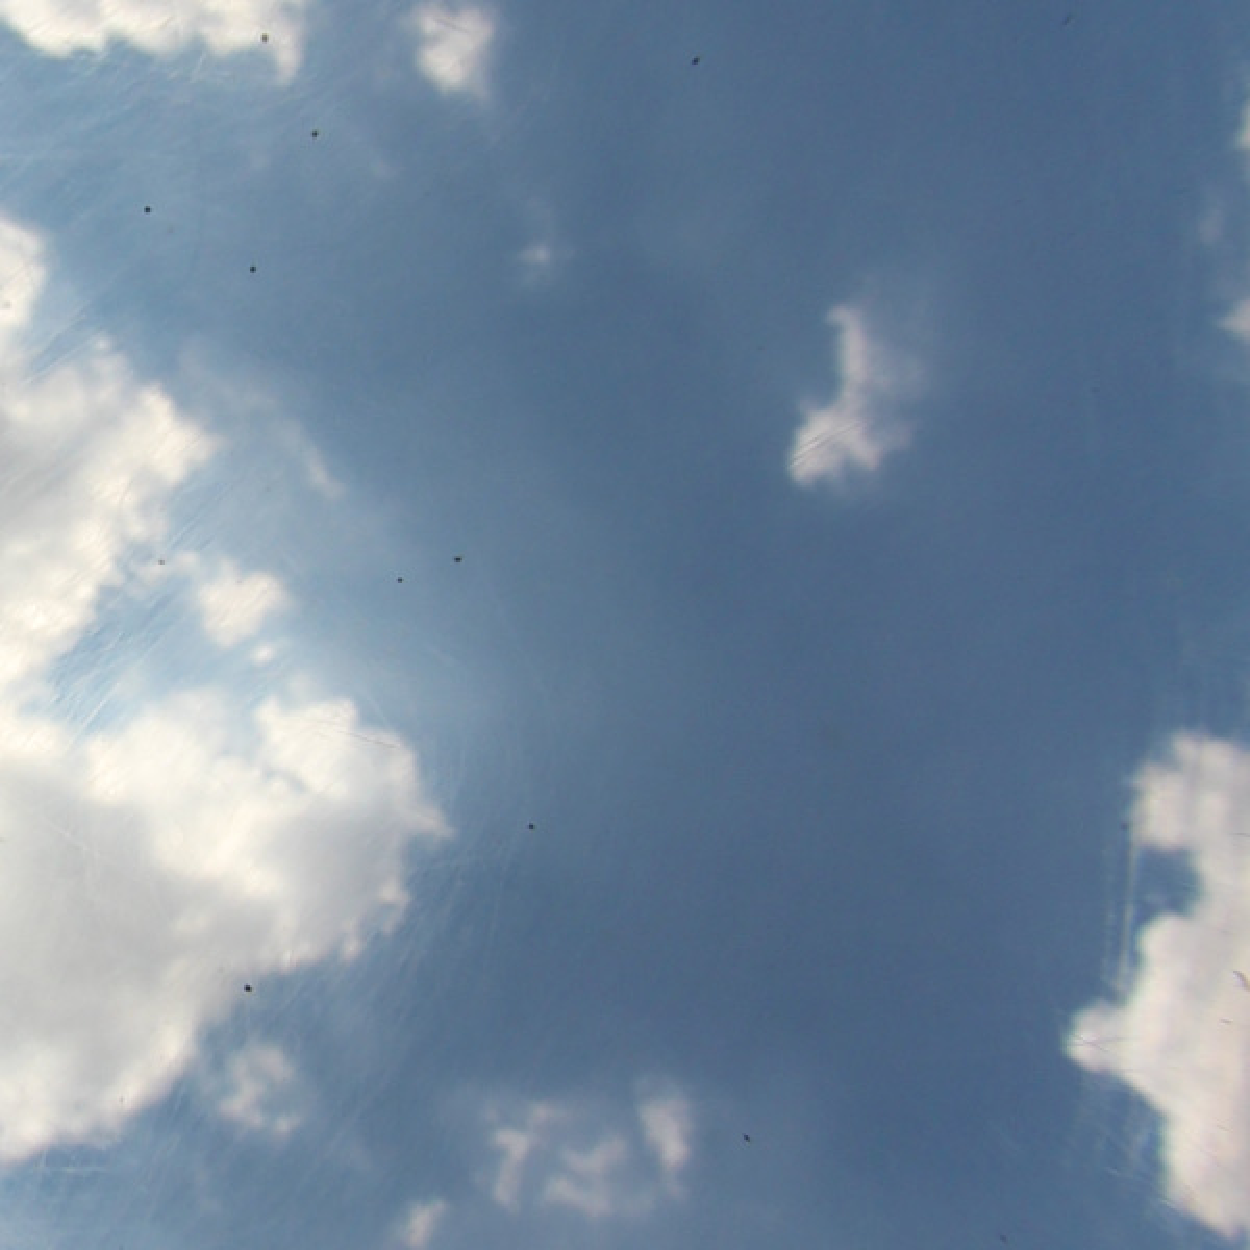
\includegraphics[height=0.08\textheight]{482img.pdf} &
\includegraphics[height=0.08\textheight]{583img.pdf} &
\includegraphics[height=0.08\textheight]{im2.pdf}& \vspace{-0.39in}\\

{\fontsize{0.4cm}{1em}\selectfont Ground Truth} \vspace{1.5cm}& 
\includegraphics[height=0.08\textheight]{B1_GT.pdf} &
\includegraphics[height=0.08\textheight]{B4_GT.pdf} &
\includegraphics[height=0.08\textheight]{C1_GT.pdf} &
\fbox{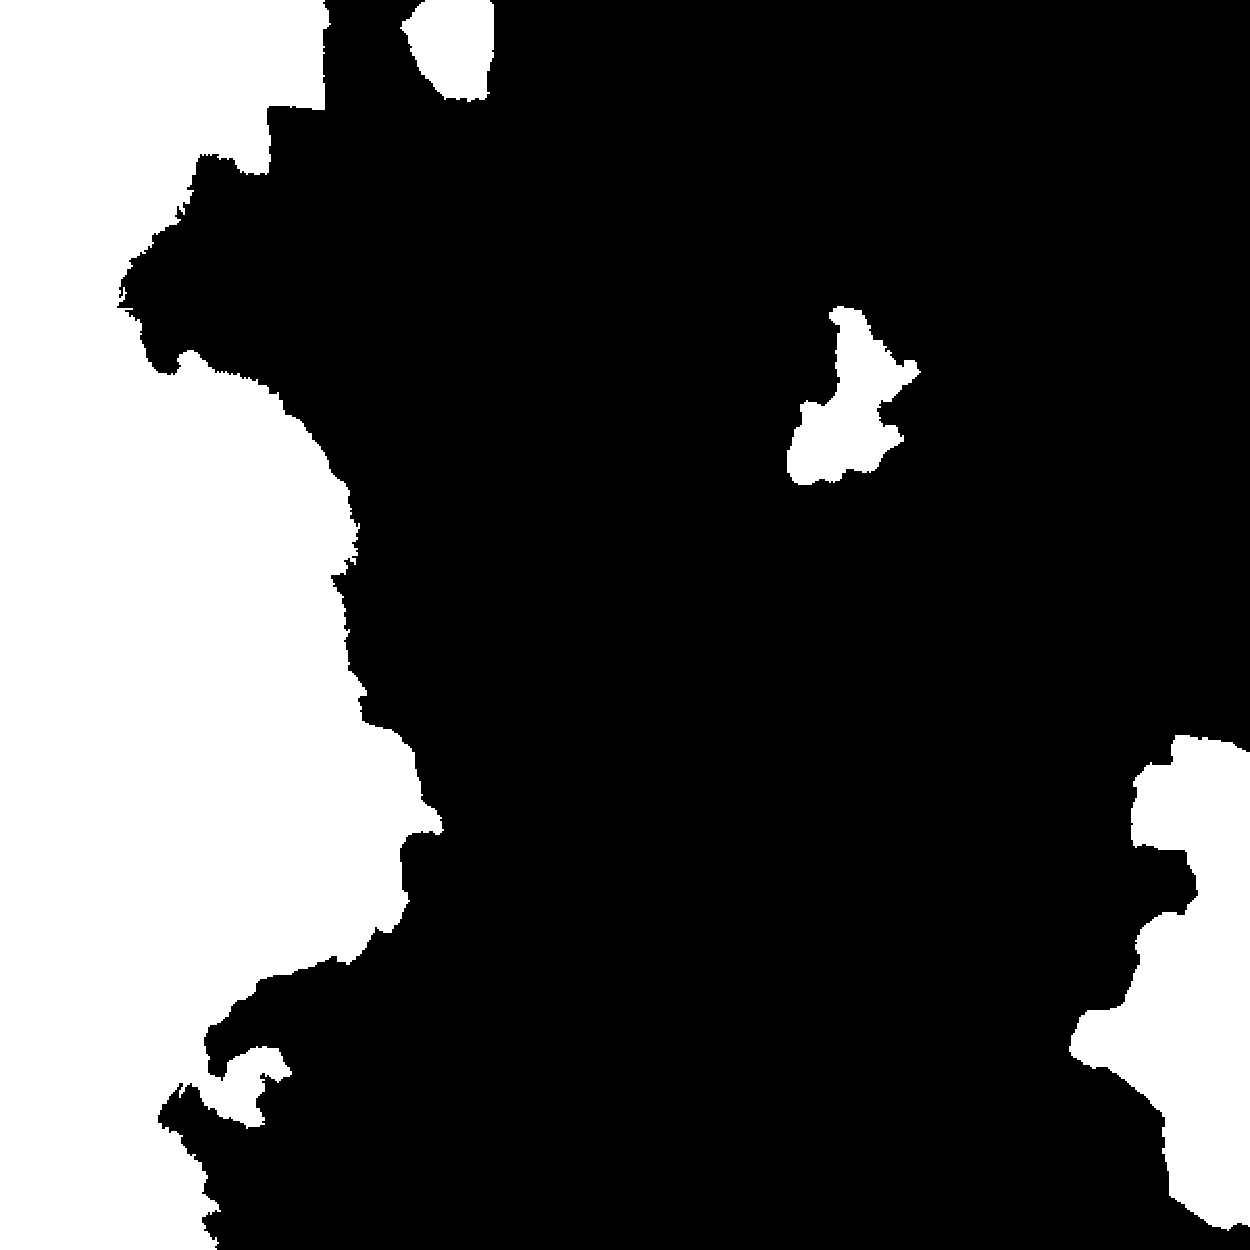
\includegraphics[height=0.08\textheight]{482img_2GT.pdf}} &
\fbox{\includegraphics[height=0.08\textheight]{583img_2GT.pdf}} &
\fbox{\includegraphics[height=0.08\textheight]{im2-GT.pdf}}& \vspace{-0.39in}\\

{\fontsize{0.4cm}{1em}\selectfont Our \mbox{approach}} \vspace{1.5cm}& 
\includegraphics[height=0.08\textheight]{B1-map.pdf} &
\includegraphics[height=0.08\textheight]{B4-map.pdf} &
\includegraphics[height=0.08\textheight]{C1-map.pdf} &
\includegraphics[height=0.08\textheight]{482img-map.pdf} &
\includegraphics[height=0.08\textheight]{583img-map.pdf} &
\includegraphics[height=0.08\textheight]{im2-prob.pdf}&
\hspace{-0.18in}\includegraphics[height=0.08\textheight]{redblue-map.pdf}\vspace{-0.39in}\\

{\fontsize{0.4cm}{1em}\selectfont Our \mbox{approach} (binary)} \vspace{1.5cm}& 
\includegraphics[height=0.08\textheight]{B1-thr.pdf} &
\includegraphics[height=0.08\textheight]{B4-thr.pdf} &
\includegraphics[height=0.08\textheight]{C1-thr.pdf} &
\fbox{\includegraphics[height=0.08\textheight]{482img-thr.pdf}} &
\fbox{\includegraphics[height=0.08\textheight]{583img-thr.pdf}} &
\fbox{\includegraphics[height=0.08\textheight]{im2-prop.pdf}}& \vspace{-0.39in}\\


{\fontsize{0.4cm}{1em}\selectfont Li et al.} \vspace{1.5cm}& 
\includegraphics[height=0.08\textheight]{B1-HYTA.pdf} &
\includegraphics[height=0.08\textheight]{B4-HYTA.pdf} &
\includegraphics[height=0.08\textheight]{C1-HYTA.pdf} &
\fbox{\includegraphics[height=0.08\textheight]{482img-HYTA.pdf}} &
\fbox{\includegraphics[height=0.08\textheight]{583img-HYTA.pdf}} &
\fbox{\includegraphics[height=0.08\textheight]{im2_li.pdf}}& \vspace{-0.33in}\\


{\fontsize{0.4cm}{1em}\selectfont Souza et al.} \vspace{1.5cm}& 
\includegraphics[height=0.08\textheight]{B1-Souza.pdf} &
\includegraphics[height=0.08\textheight]{B4-Souza.pdf} &
\includegraphics[height=0.08\textheight]{C1-Souza.pdf} &
\fbox{\includegraphics[height=0.08\textheight]{482img-Souza.pdf}} &
\fbox{\includegraphics[height=0.08\textheight]{583img-Souza.pdf}} &
\fbox{\includegraphics[height=0.08\textheight]{im2-Souza.pdf}}& \vspace{-0.37in}\\


{\fontsize{0.4cm}{1em}\selectfont Long et al.} \vspace{1.5cm}& 
\fbox{\includegraphics[height=0.08\textheight]{B1-Long.pdf}} &
\fbox{\includegraphics[height=0.08\textheight]{B4-Long.pdf}} &
\fbox{\includegraphics[height=0.08\textheight]{C1-Long.pdf}} &
\fbox{\includegraphics[height=0.08\textheight]{482img-Long.pdf}} &
\fbox{\includegraphics[height=0.08\textheight]{583img-Long.pdf}} &
\fbox{\includegraphics[height=0.08\textheight]{im2-long.pdf}}& \vspace{-0.39in}\\


{\fontsize{0.4cm}{1em}\selectfont Mantelli-Neto et al.} \vspace{1.5cm}& 
\fbox{\includegraphics[height=0.08\textheight]{B1-Syl.pdf}} &
\fbox{\includegraphics[height=0.08\textheight]{B4-Syl.pdf}} &
\includegraphics[height=0.08\textheight]{C1-Syl.pdf} &
\fbox{\includegraphics[height=0.08\textheight]{482img-Syl.pdf}} &
\fbox{\includegraphics[height=0.08\textheight]{583img-Syl.pdf}} &
\fbox{\includegraphics[height=0.08\textheight]{im2-sylvio.pdf}}& \vspace{-0.33in}\\


{\fontsize{0.4cm}{1em}\selectfont SLIC + \mbox{DBSCAN}} \vspace{1.5cm}& 
\includegraphics[height=0.08\textheight]{B1-SLIC.pdf} &
\includegraphics[height=0.08\textheight]{B4-SLIC.pdf} &
\fbox{\includegraphics[height=0.08\textheight]{C1-SLIC.pdf}} &
\fbox{\includegraphics[height=0.08\textheight]{482img-SLIC.pdf}} &
\fbox{\includegraphics[height=0.08\textheight]{583img-SLIC.pdf}} &
\fbox{\includegraphics[height=0.08\textheight]{im2-slic.pdf}}& \vspace{-0.36in}\\

{\fontsize{0.4cm}{1em}\selectfont GRAY + SVM} \vspace{1.2cm}& 
\fbox{\includegraphics[height=0.08\textheight]{B1-graySVM.pdf}} &
\includegraphics[height=0.08\textheight]{B4-graySVM.pdf} &
\fbox{\includegraphics[height=0.08\textheight]{C1-graySVM.pdf}} &
\fbox{\includegraphics[height=0.08\textheight]{482img-graySVM.pdf}} &
\fbox{\includegraphics[height=0.08\textheight]{583img-graySVM.pdf}} &
\fbox{\includegraphics[height=0.08\textheight]{im2-gray-svm.pdf}}& \vspace{-0.39in}\\


{\fontsize{0.4cm}{1em}\selectfont dSIFT + BOW + SVM} \vspace{1.5cm}& 
\fbox{\includegraphics[height=0.08\textheight]{B1-dSIFT.pdf}} &
\includegraphics[height=0.08\textheight]{B4-dSIFT.pdf} &
\fbox{\includegraphics[height=0.08\textheight]{C1-dSIFT.pdf}} &
\fbox{\includegraphics[height=0.08\textheight]{482img-dSIFT.pdf}} &
\fbox{\includegraphics[height=0.08\textheight]{583img-dSIFT.pdf}} &
\fbox{\includegraphics[height=0.08\textheight]{im2-dSIFT.pdf}}& \vspace{-0.39in}\\

\end{tabular}
\captionof{figure}[Segmentation results of sample images from HYTA and SWIMSEG databases for different benchmarking algorithms.]{Sample images from HYTA (left 3 columns) and SWIMSEG (right 3 columns) databases, along with the corresponding ground truth and the sky/cloud segmentation obtained using various methods. The \emph{blue} and \emph{red} in the colormap indicate \emph{sky} and \emph{cloud} respectively.}
\label{fig:sample-results}
\end{table}

The simulations were conducted in Matlab on a 64-bit Ubuntu 14.04 LTS workstation, Intel i5 CPU $@$2.67GHz.  In terms of computation time, our proposed method takes an average of  $1.31$s and $1.89$s for a single image from the HYTA and SWIMSEG databases, respectively. In the training stage, HYTA requires $21.5$s and SWIMSEG required $1018.6$s for computing the regression coefficient matrix $\mathbf{B}$. The computation times of other benchmarking algorithm are provided in Table~\ref{scoretable}.

Table~\ref{scoretable} provides an objective evaluation of our proposed approach with other state-of-the-art algorithms for all images in the testing set of the two databases.  Existing algorithms require extensive tuning using various manually-defined thresholds, and achieve either high precision or high recall in our evaluation, but not both. Long et al.\ and Mantelli-Neto et al.\ have high recall values. However, they fare poorly in the corresponding precision values. Souza et al.\ on the other hand has a high precision value, but low recall. These existing methods often suffer from under- or over-identification of cloud pixels as they are threshold-based, and a single threshold may not work well for all types of sky/cloud images. Our proposed approach performs best for both HYTA and SWIMSEG databases on the basis of F-scores, highlighting the effectiveness of PLS-based learning method. 

\begin{table}[htbp]
\footnotesize
\centering
\begin{tabular}{ |lr||r|r|r|c|c| }
\hline
& Methods & Precision & Recall & F-score & Misclassification rate & Time [s] \\ 
\hline\hline
\parbox[t]{3mm}{\multirow{12}{*}{\rotatebox[origin=c]{90}{\small \textbf{HYTA}}}} 
& Li et al.\ & 0.89 & 0.82 & 0.81 & 0.12 & 1.34 \\ 
& Souza et al.\ & 0.88 &  0.67 &  0.65 & 0.15 & 1.33 \\ 
& Long et al.\ & 0.64 & \textbf{0.97} & 0.71  & 0.26 & 1.22 \\ 
& Mantelli-Neto et al.\ & 0.54 & \textbf{0.97} & 0.63 & 0.44 & 1.43 \\ 
& SLIC + DBSCAN & 0.65 & 0.83 & 0.60 & 0.32 & 5.10 \\ 
& GRAY + SVM & 0.89 & 0.58 & 0.67 & 0.31 & 2.44  \\
& LBP + SVM & 0.80 & 0.65 & 0.72 & 0.22 & 4.29 \\
& ColorHIST + SVM & 0.75 & 0.74 & 0.75 & 0.21 & 2.47  \\
& dSIFT + BOW + SVM & 0.61 & 0.66 & 0.62 & 0.38 & 4.91 \\
& Texture + BOW + SVM & 0.82 & 0.62 & 0.69 & 0.25 & 2.60  \\
& Proposed Method & \textbf{0.94} & 0.80 & \textbf{0.85} & \textbf{0.10} & 1.31  \\ 
\hline\hline
\parbox[t]{3mm}{\multirow{12}{*}{\rotatebox[origin=c]{90}{\small \textbf{SWIMSEG}}}} 
& Li et al.\ & 0.90 & 0.86 & 0.88 & 0.11 & 2.06  \\ 
& Souza et al.\ & 0.95 &  0.76 &  0.81 & 0.14 & 2.04 \\ 
& Long et al.\ & 0.71 & \textbf{0.98} & 0.80 & 0.23 & 1.83  \\ 
& Mantelli-Neto et al.\ & 0.70 & 0.97 & 0.79 & 0.24 & 2.16 \\ 
& SLIC + DBSCAN & 0.72 & 0.79 & 0.65 & 0.33 & 5.39 \\ 
& GRAY + SVM & 0.87 & 0.56 & 0.64 & 0.33 & 2.61 \\
& LBP + SVM & 0.62 & 0.65 &  0.63 & 0.36 & 4.73 \\
& ColorHIST + SVM & 0.81 & 0.64 & 0.66 & 0.31 & 2.63  \\
& dSIFT + BOW + SVM & 0.65 & 0.88 & 0.72 & 0.28 & 5.04 \\
& Texture + BOW + SVM & 0.82 & 0.71 & 0.70 & 0.31 & 2.74  \\
& Proposed Method  & \textbf{0.92} & 0.90 & \textbf{0.90} & \textbf{0.09} & 1.89 \\ 
\hline
\end{tabular}
\caption[Performance evaluation of different benchmarking algorithms.]{Performance evaluation using binary ground truth of HYTA and SWIMSEG databases. The best performance according to each criterion is indicated in bold. All experiments are evaluated on the same set of testing images from the HYTA and SWIMSEG databases. We also list the computation time for a single image for all algorithms.}
\label{scoretable}
\end{table}


\section{High-Dynamic-Range Imaging for Cloud Segmentation}
\label{sec:HDRI-segment}
While there have been several studies analyzing clouds and their features from WSI images~\cite{Long,Souza,Li2011,LiuSP2015,ICIP1_2014}, most of them avoid the circumsolar region, because capturing the details in this area is a non-trivial task. In this section, we show how to improve segmentation results by capturing a larger dynamic range of the sky using High-Dynamic-Range Imaging (HDRI) techniques. We then introduce HDRSeg, a graph-cut based segmentation algorithm that uses the HDR radiance map for accurate segmentation of sky/cloud images. Figure~\ref{fig:story-HDRSeg} briefly summarizes our proposed approach.

\begin{figure}[htb]
\centering
\includegraphics[width=0.18\textwidth]{LDR1-E}\hspace{0.5mm}    
\includegraphics[width=0.18\textwidth]{LDR2-E}\hspace{0.5mm} 
\includegraphics[width=0.18\textwidth]{LDR3-E}\hspace{0.5mm}
\includegraphics[width=0.18\textwidth]{tonemapped-E}\hspace{0.5mm}
\includegraphics[width=0.18\textwidth]{binary-E}\hspace{0.5mm}\\
\makebox[0.18\textwidth][c]{(a)}
\makebox[0.18\textwidth][c]{(b)}
\makebox[0.18\textwidth][c]{(c)}
\makebox[0.18\textwidth][c]{(d)}
\makebox[0.18\textwidth][c]{(e)}
\caption[Proposed HDRSeg cloud segmentation approach.]{Proposed HDRSeg cloud segmentation approach. (a) High- (b) Mid- (c) Low-exposure Low-Dynamic-Range (LDR) images; (d) Tonemapped High-Dynamic-Range (HDR) image; (e) Binary output using HDRSeg. Saturated pixels in all images are shown in pink. The number of saturated pixels is significantly reduced in the tonemapped HDR image, without compromising on the fine cloud details.}
\label{fig:story-HDRSeg}
\end{figure}


The motivation is to propose the use of HDR imaging for cloud segmentation in ground-based sky cameras. We have already detailed the process of image capture and storage in our sky camera system an earlier Chapter~\ref{chap:wsi} of this thesis. We showed that using HDR images for cloud imaging significantly reduces the amount of saturated pixels in an image, and is therefore an efficient manner to capture the circumsolar region. Furthermore, HDR imaging generally provides better segmentation results, as compared to LDR images, regardless of the segmentation method used.



\subsection{Cloud Segmentation Using HDRI}
We propose a graph-based segmentation algorithm called HDRSeg, that formulates the sky/cloud segmentation task as a graph-partitioning problem. Graph-cut for cloud segmentation was proposed earlier by Liu et al.~\cite{Liu_AGC}. However, Liu et al.\ used conventional LDR images in their segmentation framework and generated seeds using Otsu threshold~\cite{Otsu79}. Also, they did not consider the circumsolar regions in their evaluation.

\subsubsection{Notations}
Suppose that the low-, mid- and high-exposure LDR sky/cloud images are represented by $\mathbf{Z}_i^{L}$, $\mathbf{Z}_i^{M}$ and $\mathbf{Z}_i^{H}$ respectively, $i=1,\ldots,N_h$, where $N_h$ is the total number of HDR sets in the dataset. Without any loss of generality, $\mathbf{Z}_i$ denotes either low-, mid- or high-exposure LDR image in the subsequent sections. Each of these LDR images are \emph{RGB} color images, $\mathbf{Z}_i \in {\rm I\!\mathbf{R}}^{m \times n \times 3}$, having a dimension $m \times n$ for each \emph{R}, \emph{G} and \emph{B} channels. We generate the HDR radiance map $\mathcal{H}_i \in {\rm I\!\mathbf{R}}^{m \times n \times 3}$ from the set of three LDR images $\mathbf{Z}_i^{L}$, $\mathbf{Z}_i^{M}$ and $\mathbf{Z}_i^{H}$, as described in Section~\ref{sec:HDR-discuss}. 

Let $\tilde{p}$ be a sample pixel in the image $\mathbf{Z}_i$. We aim to assign labels to each of the pixels $\tilde{p}$, as either \emph{cloud} or \emph{sky}. We denote the label as $L_{\tilde{p}}$, where $L_{\tilde{p}} = 1 \mbox{ or } 0$ if $\tilde{p}$ is a \emph{cloud} or \emph{sky} pixel, respectively. We model this task as a graph-based discrete labeling problem, wherein we represent $\mathbf{Z}_i$ as a graph, comprising a set of nodes and edges.

\subsubsection{Generating Seeds}
Graph-cut based segmentation algorithms~\cite{Boykov_ICCV} require the user to initially label a few pixels as 'foreground' and 'background'.   We refer to these prior labeled pixels as \emph{seeds}. The process of generating seeds is generally done manually before partitioning the graph into two sub-graphs. In HDRSeg, we automatically generate these initial seeds by assigning a few pixels in the sky/cloud image with \emph{sky} and \emph{cloud} labels. 

In our previous Chapter~\ref{chap:colorchannels}, we have performed a systematic analysis of the existing color spaces and components, and observed that $(B-R)/(B+R)$ is one of the most discriminating color channels for cloud segmentation ($B$ and $R$ indicate the blue and red channels of the image). Furthermore, in this current chapter, we have proposed a probabilistic approach for sky/cloud image segmentation, instead of the conventional binary approach. In this probabilistic approach, each pixel is assigned a \emph{soft} membership to belong to \emph{cloud} category, instead of a \emph{hard} membership. 

To illustrate these concepts, consider the example shown in Fig.~\ref{fig:see-seeds}. Figure~\ref{fig:see-seeds}(a) shows a sample LDR sky/cloud image $\mathbf{Z}_i$. We extract the $(B-R)/(B+R)$ color channel from this LDR image and show it in Fig.~\ref{fig:see-seeds}(b). A fuzzy c-means clustering on this extracted color channel yields the probabilistic output image, shown in Fig.~\ref{fig:see-seeds}(c). It denotes the confidence level of each pixel to belong to the cloud category. We assume that for a given pixel, the sum of membership values for sky and cloud category is unity.

\begin{figure}[htb]
\centering
\includegraphics[height=0.28\textwidth]{mid-expo}\hspace{0.5mm}    
\includegraphics[height=0.28\textwidth]{BR}\hspace{0.5mm} 
\includegraphics[height=0.28\textwidth]{BR_block_v2}\hspace{0.5mm}\\
\makebox[0.3\textwidth][c]{(a)}
\makebox[0.3\textwidth][c]{(b)}
\makebox[0.3\textwidth][c]{(c)}
\caption[Illustrative example to show the ratio image and probabilistic segmented image.]{Illustrative example to demonstrate the probability of a pixel belonging to the `cloud' category. (a) Sample sky/cloud image; (b) $(B-R)/(B+R)$ color channel image; (c) Probabilistic output image using the method described in Section~\ref{sec:prob-segment}.}
\label{fig:see-seeds}
\end{figure}

In HDRSeg, we apply fuzzy c-means clustering to the $(B-R)/(B+R)$ ratio channel of the HDR radiance map $\mathcal{H}_i$ to estimate the probability of a pixel belonging to the cloud category. We denote the ratio channel as $\tilde{\mathcal{R}}_i$. The membership values obtained by clustering provide us a mechanism in assigning the seeds with a degree of confidence. We assign these initial seeds for HDRSeg as follows: pixels having membership \textgreater $\tilde{\alpha}$ and \textless $(1-{\tilde{\alpha}})$ are labeled as cloud and sky respectively. The value of $\tilde{\alpha}$ is a constant and is set experimentally (more on this below).

\subsubsection{Partitioning the HDR Graph}
The segmentation framework of HDRSeg employs a graph-based image segmentation approach, wherein we represent the ratio-image $\tilde{\mathcal{R}}_i \in {\rm I\!\mathbf{R}}^{m \times n}$ as a set of nodes and edges. Each edge of the graph is given a corresponding weight that measures the dissimilarity between two pixels. We follow the work of Boykov and Jolly~\cite{Boykov_ICCV} and try to minimize the segmentation score $E$:
\begin{equation}\label{eq:agc}
\begin{aligned}
E=\sum_{\tilde{p}}^{}  A_{\tilde{p}} +\mu \sum_{(\tilde{p},\tilde{q}) \in \tilde{\mathcal{N}} ; A_{\tilde{p}} \neq A_{\tilde{q}}}^{}B_{\tilde{p},\tilde{q}},
\end{aligned}
\end{equation}
where $A_{\tilde{p}}$ denotes the data cost for an individual pixel $\tilde{p}$, $B_{\tilde{p},\tilde{q}}$ denotes the interaction cost between two neighboring pixels $\tilde{p}$ and $\tilde{q}$ in a small neighborhood $\tilde{\mathcal{N}}$, and $\mu$ is the weighting parameter.




The complete proposed HDR segmentation algorithm can be summarized as follows:

\begin{algorithm}[htb]
\caption{HDRSeg}
\label{alg:HDRSegalgo} 
\begin{algorithmic}[1]
\Require LDR sky/cloud images with varying EVs.
\Ensure Segmented image.
\State Create HDR radiance map $\mathcal{H}_i$ from bracketted set of LDR images;
\State Extract $(B-R)/(B+R)$ ratio channel $\tilde{\mathcal{R}}_i$ from HDR radiance map $\mathcal{H}_i$;
\State Generate initial seeds from extracted ratio channel for image segmentation;
\State Partition the ratio channel $\tilde{\mathcal{R}}_i$ into two subgraphs using the generated seeds;
\State \textbf{return} Binary segmented image.
\end{algorithmic}
\end{algorithm}


We illustrate the complete HDRSeg segmentation framework in Fig.~\ref{fig:HDRcut}. Figure~\ref{fig:HDRcut}(a) represent the three sample LDR images $\mathbf{Z}_i^{L}$, $\mathbf{Z}_i^{M}$ and $\mathbf{Z}_i^{H}$ respectively captured at $\{-4,-2,0\}$ EV settings. We generate the corresponding HDR radiance map $\mathcal{H}_i$ from these LDR images. A tone-mapped version of $\mathcal{H}_i$ is shown in Fig.~\ref{fig:HDRcut}(b), for visualization purposes. We extract the $(B-R)/(B+R)$ ratio channel from $\mathcal{H}_i$, and generate the initial cloud and sky seeds marked in \emph{green} and \emph{red} color respectively, as shown in Fig.~\ref{fig:HDRcut}(c). The binary output image after graph cut is shown in Fig.~\ref{fig:HDRcut}(d).


\begin{figure}[htb]
\centering
\includegraphics[width=0.15\textwidth]{low-expo}\hspace{0.5mm}    
\includegraphics[width=0.15\textwidth]{mid-expo}\hspace{0.5mm} 
\includegraphics[width=0.15\textwidth]{high-expo}\hspace{0.5mm}
\includegraphics[width=0.15\textwidth]{HDR-tonemap}\hspace{0.5mm}
\includegraphics[width=0.15\textwidth]{seeded-image_v2}\hspace{0.5mm}
\includegraphics[width=0.15\textwidth]{binary-mask}\hspace{0.5mm}\\
\makebox[0.15\textwidth][c]{(a-i)}
\makebox[0.15\textwidth][c]{(a-ii)}
\makebox[0.15\textwidth][c]{(a-iii)}
\makebox[0.15\textwidth][c]{(b)}
\makebox[0.15\textwidth][c]{(c)}
\makebox[0.15\textwidth][c]{(d)}
\caption[Illustrating explaining the proposed HDRSeg framework.]{Proposed HDRSeg framework for sky/cloud segmentation. (a) Exposure bracketed $\{-4,-2,0\}$ Exposure Value (EV) LDR images; (b) High Dynamic Range (HDR) image tone-mapped for visualization purpose; (c) Image with initial seeds, where \emph{cloud} seeds and \emph{sky} seeds are represented in \emph{green} and \emph{red} respectively, and undecided pixels are represented in \emph{yellow}; (d) Binary sky/cloud segmentation result. The saturated pixels in (b), (c) and (d) are masked in pink.}
\label{fig:HDRcut}
\end{figure}



\subsection{Experimental Evaluation}

\subsubsection{HDR Sky/Cloud Image Database}
Currently there are no available HDR image datasets for sky/cloud images. We therefore consider $26$ sets of HDR captures, which comprise a total of $78$ LDR images. Each HDR capture is based on three LDR images (low- ,mid- and high-) which were captured in Automatic Exposure Bracketing (AEB) mode of our camera. These high-quality HDR images are captured with our sky imagers, which we cropped to remove the occlusions by buildings or antennas near the horizon line. The average dimension of the captured LDR images is of $1800 \times 1600$ pixels. They were captured at various times of the day, under different weather conditions. The corresponding ground truth images were manually generated in consultation with experts from the Meteorological Service Singapore (MSS). We perform a detailed evaluation of several cloud segmentation algorithms on this newly created dataset. 

\subsubsection{Results}
HDR imaging is an effective technique for cloud observation. It helps us better image the circumsolar region, without saturating the neighboring pixels. To illustrate this fact, we calculate the number of saturated pixels in the low-, med- and high- LDR images. We also calculate the number of saturated pixels (if any) in tonemapped images, in the dataset. Using our HDR techniques, we observe that the tonemapped images have $87.2$ times fewer saturated pixels, as compared to the high-exposure LDR images. Similarly, it has $9.5$ times and $2.0$ times fewer saturated pixels with respect to mid- and low-exposure LDR images.

In addition to containing fewer saturated pixels, HDR imaging also helps in improved cloud segmentation performance, regardless of the techniques used, as we demonstrate in the following. 
Cloud segmentation is essentially a binary classification problem, wherein we classify each pixel as either sky or cloud labels. We report the Precision, Recall and Error values for the different cloud segmentation methods. A detailed definition of these metrics are already provided earlier in Section~\ref{sec:result-segment}. 

For evaluation purposes, we benchmark HDRSeg with existing cloud segmentation algorithms. We consider Li et al.~\cite{Li2011}, Long et al.~\cite{Long}, Souza et al.~\cite{Souza} and Mantelli-Neto et al.~\cite{Sylvio}. All these existing algorithms, which were briefly described in Chapter~\ref{chap:litreview}, are designed for conventional LDR images.

We designed our proposed HDRSeg segmentation algorithm on the HDR radiance maps. We extract the $(B-R)/(B+R)$ channel from these high-dynamic radiance maps, and assign the initial seeds for \emph{cloud} and \emph{sky} pixels. The value of $\tilde{\alpha}$ determines the amount of initial seeds in HDRSeg. We empirically set the value of $\tilde{\alpha}$ to $0.98$. We set a high value of $\tilde{\alpha}$, because it corresponds to higher confidence in assigning the correct labels.

Since existing cloud segmentation algorithms are designed for conventional LDR images, we evaluate these current cloud segmentation algorithms on the mid-exposure LDR images as well as the tonemapped images. Our proposed HDRSeg algorithm is the only one designed to make use of the full HDR radiance maps. However, for the sake of comparison, we also evaluate for mid-exposure LDR and tonemapped images. The detailed evaluation results of HDRSeg, along with the other cloud segmentation algorithms, are shown in Table~\ref{tab:scores}.

\begin{table}[htb] % start table environment
\footnotesize
\begin{center} % center the table and caption
% build the table
\begin{tabular}{p{2.2cm}|p{1cm}p{1cm}p{1cm}|p{1cm}p{1cm}p{1.5cm}|p{1cm}p{1cm}p{1.5cm}}
& \multicolumn{3}{c}{Using LDR image} & \multicolumn{3}{c}{Using Tonemapped image} 
			& \multicolumn{3}{c}{Using HDR Luminance map} \\
Methods & \scriptsize{Precision} & \scriptsize{Recall} & \scriptsize{Error [\%]} & \scriptsize{Precision} & \scriptsize{Recall} & \scriptsize{Error [\%]} & \scriptsize{Precision} & \scriptsize{Recall} & \scriptsize{Error [\%]}\\
\hline
Long et al.\ & 0.68 & 0.99 & 31.77 & 0.72 & 0.99 & 27.31 ($\uparrow$) & - & - & -\\
Souza et al.\ & 0.76 & 0.99 & 21.80 & 0.79 & 0.95 & 20.98 ($\uparrow$) & - & - & -\\
Mantelli-Neto et al.\ & 0.69 & \textbf{1.0} & 31.33 & 0.84 & \textbf{1.0} & 15.41 ($\uparrow$) & - & - & -\\
Li et al.\ & 0.90 & 0.90 & 11.93 & 0.79 & 0.92 & 24.45 ($\downarrow$) & - & - & -\\
HDRSeg & 0.77 & 0.98 & 21.12 & 0.81 & 0.95 & 18.93 ($\uparrow$) & \textbf{0.95} & 0.88 & \textbf{10.44} ($\uparrow$) \\
\hline
\end{tabular}
\caption[Comparison of HDRSeg segmentation algorithms with other benchmarking algorithms.]{The average scores across all the images are reported for the various benchmark methods. The \emph{arrow} inside the parenthesis indicates the error performance of the algorithm as compared to its corresponding LDR version. We indicate increase (and decrease) in performance with $\uparrow$ (and $\downarrow$) respectively, when compared with LDR image. The best performance according to each criterion is indicated in bold.} % caption for the table (gives it a number)
\label{tab:scores}
\end{center}
\end{table}


From Table~\ref{tab:scores}, we observe that HDR imaging improves the cloud segmentation performance, irrespective of the methods used. We observe that most of the benchmark algorithms (except for Li et al.) have a better performance with tonemapped images, as compared to mid-exposure LDR image. This is because a tonemapped version exhibits fewer saturated pixels and clearer contrast between sky and cloud, as compared to the corresponding LDR image. However, HDRSeg using the entire HDR luminance map achieves the best error performance of $10.44 \%$ across all the methods.

Most of the other algorithms are biased towards a higher recall value (tendency to over-estimate cloud cover), as compared to precision. These existing algorithms are based on a set of thresholds, either fixed or adaptive, and are therefore more prone to high error percentage. However, HDRSeg uses the entire dynamic range of sky/cloud scenes to make a more informed decision in classifying a pixel as cloud or sky. 


\section{Conclusions}
\label{sec:conc}
There are three primary advantages of our proposed segmentation approach compared to other cloud detection algorithms.

First, our cloud segmentation framework is not based on any pre-defined assumptions about color spaces and does not place any restrictions on the type of input images.  We systematically compare different color channels and identify the most suitable ones. We also explain the reason for their better performance based on rigorous statistical evaluations in two datasets. 

Second, many existing cloud segmentation algorithms rely on a set of thresholds, conditions, and/or parameters that are manually defined for a particular sky/cloud image database. Our proposed cloud segmentation approach is entirely learning-based and thus provides a systematic solution to training for a given database. 

Third, conventional algorithms provide a binary output image from the input sky/cloud image. Although these binary images are informative in most cases, they lack flexibility and robustness. We have no indication of the effectiveness of the thresholding of the input image. In reality, because of the nature of clouds and cloud images, it is undoubtedly better to employ a \emph{soft} thresholding approach. Our proposed approach achieves a probabilistic classification of cloud pixels. This is very informative as it provides a general sense of \emph{belongingness} of pixels to the cloud class. However, as only binary ground-truth images are available, we convert these probability maps into binary images for performing a quantitative evaluation of our algorithm. In our future work, we plan to extend this analysis by creating \emph{probabilistic ground truth} images, where the ground truth of the input images is generated by aggregating  annotations from multiple experts.

Finally, from the extensive experiments on the two datasets (cf.\ Table~\ref{scoretable}), we observe that the performance with images from the SWIMSEG database is generally better than for HYTA, even though the behavior of color channels is similar in both (i.e.\ the same color channels do well for both SWIMSEG and HYTA).  We believe this is because the images in SWIMSEG were captured with a camera that has been calibrated for color, illumination, and geometry~\cite{WAHRSIS}. 

Naturally, many challenges remain, for example: How do different weather conditions affect the classification performance?  The weather in Singapore is relatively constant in terms of temperature and humidity, with little variation throughout the year.  Usually it is either partly cloudy, or rainy (in which case the sky will be completely overcast, making segmentation unnecessary). As a result, our database is not suitable for investigating this question. Completely overcast conditions can be dealt with by simple pre-processing of the image before segmentation, e.g.\ by calculating the number of clusters, as we have done in our previous work~\cite{ICIP2015a}. 


In this chapter, we have proposed a probabilistic approach using PLS-based regression for the segmentation of ground-based sky/cloud images. Our approach is entirely learning-based and does not require any manually-defined thresholds, conditions, or parameters at any stage of the algorithm. We also release an extensive sky/cloud image database captured with a calibrated ground-based camera that has been annotated with ground-truth segmentation masks. The conventional segmentation techniques are not catered for the circumsolar region, as those particular images are completely saturated. In the later part of this chapter, we solved the cloud segmentation problem for images around the sun using HDRI techniques.

Our future work will include the annotation of a database with probabilistic ground-truth segmentation maps. In the following chapters, we will go beyond segmentation, and devise algorithms to classify clouds into different types~\cite{ICIP2015a}. Also, we will provide theoretical studies in estimating cloud base height for multi-camera setups. 




